% Schematic mode clocks for the printed two-by-two example; not a solved trajectory.
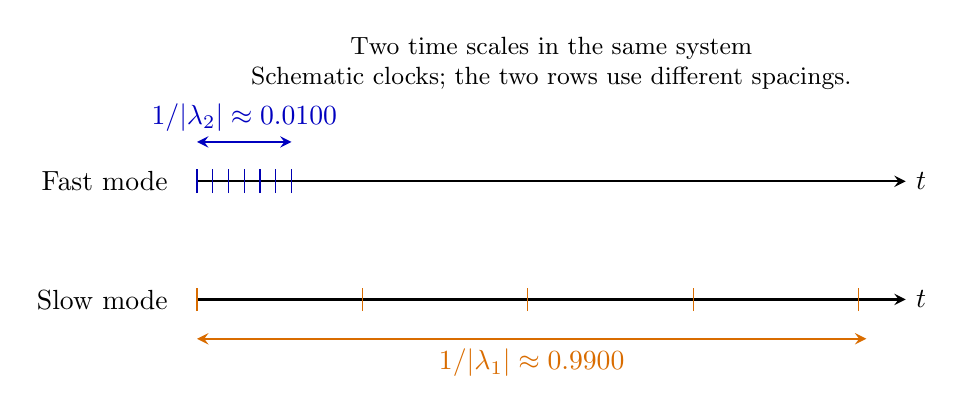
\begin{tikzpicture}[>=stealth,font=\normalsize]
\draw[->,thick](0,1.5)--(9,1.5)node[right]{$t$};
\draw[->,thick](0,0)--(9,0)node[right]{$t$};
\node[anchor=east]at(-.25,1.5){Fast mode};\node[anchor=east]at(-.25,0){Slow mode};
\draw[<->,blue!75!black,thick](0,2)--node[above]{$1/|\lambda_2|\approx0.0100$}(1.2,2);
\draw[<->,orange!85!black,thick](0,-.5)--node[below]{$1/|\lambda_1|\approx0.9900$}(8.5,-.5);
\foreach \x in {0,.2,.4,.6,.8,1,1.2}{\draw[blue!70!black](\x,1.35)--(\x,1.65);}
\foreach \x in {0,2.1,4.2,6.3,8.4}{\draw[orange!85!black](\x,-.15)--(\x,.15);}
\node[font=\small,align=center]at(4.5,3){Two time scales in the same system\\Schematic clocks; the two rows use different spacings.};
\end{tikzpicture}
